\documentclass[a4,12pt]{scrartcl}

%Basic 
\usepackage[utf8]{inputenc}
\usepackage[ngerman]{babel}
\usepackage[T1]{fontenc}
\usepackage{float}
\usepackage[bottom = 3.50cm]{geometry}

%Titel Seite
\title{CLOUD INFRASTRUCTURE}
\subtitle{Lab-10}
\author{Giorgio Vincenti \and Samuel Krieg}
\date{\today}


%Kopf, Fusszeile
\usepackage{fancyhdr}
\pagestyle{fancy}
\lhead{ \begin{picture}(0,0) \put(0,0){
\includegraphics[width=3cm]{./pictures/hsrlogo.png}} \end{picture}}
\chead{}
\rhead{Seite \thepage}
\lfoot{Cloud Infrastructure \\Lab-10}
\cfoot{Giorgio Vincenti \and Samuel Krieg}
\rfoot{\today}
\renewcommand{\headrulewidth}{0.4pt}

%Bilder
\usepackage{graphicx}

%Tabellen
\usepackage{booktabs}

%Codesnippets
\usepackage{listings}
\lstset{language=python} 

%Hyperlinks
\usepackage{hyperref}

%Querformat für eine Seite
\usepackage{lscape}
\usepackage{rotating}
\usepackage{pdflscape}

%Temp
\usepackage{lipsum}



\begin{document}

\clearpage\maketitle
\thispagestyle{empty}
\tableofcontents
\newpage

\section{Vorbereitung und Allgemeines}
Hier einige Dinge die zur Vorbereitung notwendig sind, um die Aufgaben erfüllen zu können. Es werden auch Befehle die zu jeder Aufgabe notwendig sind in diesem Kapitel erwähnt. 

\subsection{Infrastruktur}
Um die Aufgabe zu realisieren haben wir eine Ubuntu x64 VM verwendet. 
Auf dieser VM wird ebenfalls einiges benötigt. 
\begin{itemize}
\item Mininet 
\item Ryu (per Github, oder mit Hilfe von pip) 
\item Open vSwitch
\item Python Script pro Aufgabe (selber programmiert) 
\item Wireshark (mit OpenFlow Plugin)
\item Ryubook.pdf 
\end{itemize}

\subsection{Mininet starten}
Mininet starten um die Umgebung zu simulieren. Folgeder Befehl erstellt eine simulierte Netzwerk Infrastruktur. Dieser Befehl muss auf der Ubuntu VM als root ausgeführt werden. Dieser Befehl kann je nach Aufgabe variieren. 
\begin{lstlisting}
sudo mn --topo single,3 --mac --switch ovsk --controller remote -x
\end{lstlisting}
\begin{figure} [H]
	\begin{center}
	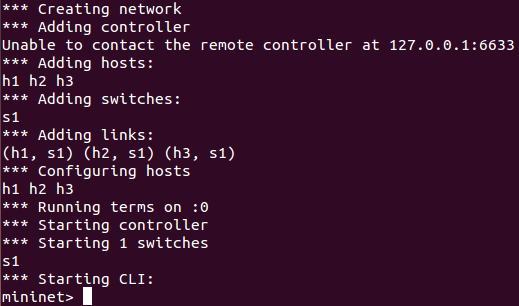
\includegraphics[width=0.40\textwidth]{./pictures/mininet.png}
	\caption{Mininet start}
	\label{x}
	\end{center}
\end{figure} 

\subsection{OpenFlow}
Hier teilen wir der Bridge mit welche OpenFlow Version verwendet werden soll. Dieser Befehl muss auf s1 ausgeführt werden. 
\begin{lstlisting}
ovs-vsctl set Bridge s1 protocols=OpenFlow13
\end{lstlisting}

\subsection{Ryu application starten}
Nachdem die obigen Vorbereitungen getroffen wurden, können wir jetzt Ryu starten mit dem erstelltem Script als Parameter. Dieser Befehl muss auf dem erstelltem Controller c0 ausgeführt werden. Auch dieser Befehl kann je nach Aufgabe variieren. (Beispiel Ryu Start aus Aufgabe 1) 
\begin{lstlisting}
ryu-manager --verbose ex1_simple_hub.py
\end{lstlisting}
\begin{figure} [H]
	\begin{center}
	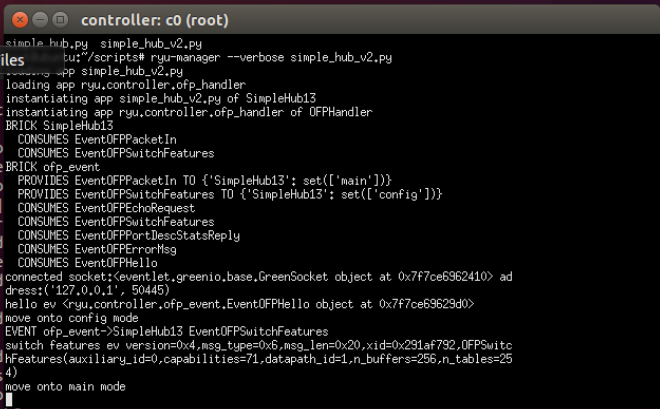
\includegraphics[width=0.50\textwidth]{./pictures/ryu_start_simple_hub.png}
	\caption{Ryu application start}
	\label{x}
	\end{center}
\end{figure} 

\subsection{Flow Table anzeigen}
Befehl auf s1 ausführen um die Flow Table anzuzeigen. 
\begin{lstlisting}
ovs-ofctl -O OpenFlow13 dump-flows s1
\end{lstlisting}
\newpage

\section{Implementing a Hub - Part 1}

\subsection{Aufgabenstellung}
Wurde aus der Aufgabenstellung entnommen: \\
\\
To get familiar with SDN controller programming you will start with a very basic and easy implementation task. The goal of this exercise is to write a hub.
\begin{itemize}
\item OpenFlow-Switch with Hub behavior
\item Each incoming packet on the OpenFlow-Switch generates a request which will be send to your SDN controller
\item The SDN controller responds to each request with a "FLOOD"-message.
\end{itemize}

\subsection{Ziel der Aufgabe}
Jeder Traffic soll über den Controller gehen, mittels OpenFlow. 

\subsection{Script: Simple Hub}
\begin{lstlisting}
#!/usr/bin/env python
from ryu.base import app_manager
from ryu.controller import ofp_event
from ryu.controller.handler import CONFIG_DISPATCHER, MAIN_DISPATCHER
from ryu.controller.handler import set_ev_cls
from ryu.ofproto import ofproto_v1_3
from ryu.lib.packet import packet

class SimpleHub13(app_manager.RyuApp):
    OFP_VERSIONS = [ofproto_v1_3.OFP_VERSION]

    def __init__(self, *args, **kwargs):
        super(SimpleHub13, self).__init__(*args, **kwargs)

    @set_ev_cls(ofp_event.EventOFPSwitchFeatures, CONFIG_DISPATCHER)
    def switch_features_handler(self, ev):
        datapath = ev.msg.datapath
        ofproto = datapath.ofproto
        parser = datapath.ofproto_parser
        match = parser.OFPMatch()
        actions = [parser.OFPActionOutput(ofproto.OFPP_CONTROLLER, 
        		ofproto.OFPCML_NO_BUFFER)]
        self.add_flow(datapath, 0, match, actions)

    def add_flow(self, datapath, priority, match, actions):
        ofproto = datapath.ofproto
        parser = datapath.ofproto_parser
        inst = [parser.OFPInstructionActions(
        			ofproto.OFPIT_APPLY_ACTIONS, actions)]
        mod = parser.OFPFlowMod(datapath=datapath, priority=priority, 
        				match=match, instructions=inst)
        datapath.send_msg(mod)

    @set_ev_cls(ofp_event.EventOFPPacketIn, MAIN_DISPATCHER)
    def _packet_in_handler(self, ev):
        msg = ev.msg
        datapath = msg.datapath
        ofproto = datapath.ofproto
        parser = datapath.ofproto_parser
        in_port = msg.match['in_port']
        out_port = ofproto.OFPP_FLOOD
        actions = [parser.OFPActionOutput(out_port)]

        data = None
        if msg.buffer_id == ofproto.OFP_NO_BUFFER:
            data = msg.data

        out = parser.OFPPacketOut(datapath=datapath, 
        	buffer_id=msg.buffer_id, in_port=in_port, 
        		actions=actions, data=data)
        datapath.send_msg(out)
        dpid = datapath.id
        self.logger.info("packet in %s %s", dpid, in_port)
\end{lstlisting}
\newpage

\subsection{Traffic}
Nachdem alles gestartet wurde können wir im Mininet von Host (h1) zu Host (h3) pingen um zu sehen ob der Verkehr mittels OpenFlow fliesst. Der Verkehr können wir mit Hilfe von Wireshark sniffen. Der gesamte Traffic verläuft über den Controller c0. Jedes Paket wird in ein OpenFlow Paket gekapselt und weitergeleitet. Der Hub ist nicht in der Lage einen Flow zu lernen. 
\begin{figure} [H]
	\begin{center}
	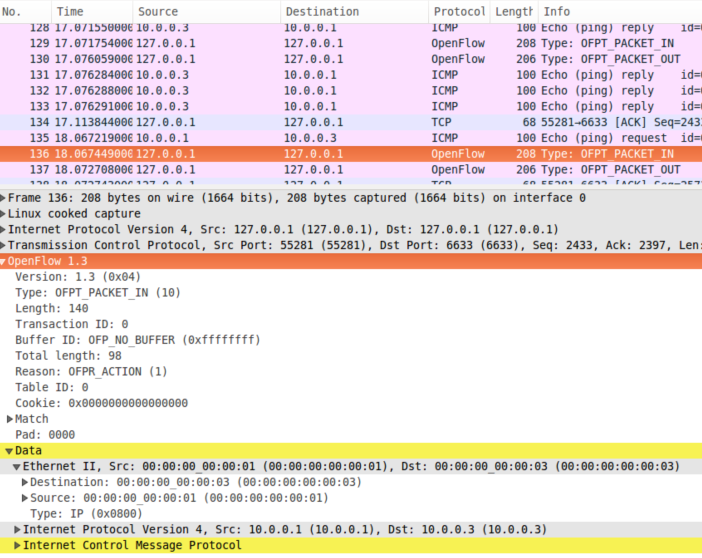
\includegraphics[width=1.00\textwidth]{./pictures/simple_hub_traffic.png}
	\caption{Mininet Traffic ping from h1 to h3}
	\label{x}
	\end{center}
\end{figure} 
\newpage

\subsection{c0 flow}
Auf der Konsole des Controllers c0 ist ersichtlich das alle Pakete zu ihm geschickt wird. 
\begin{figure} [H]
	\begin{center}
	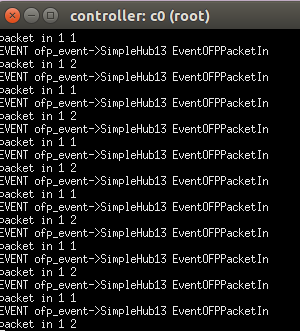
\includegraphics[width=0.60\textwidth]{./pictures/c0_ex1.png}
	\caption{c0 flow}
	\label{x}
	\end{center}
\end{figure} 
\newpage

\section{Implementing a Hub - Part 2}

\subsection{Aufgabenstellung}
Wurde aus der Aufgabenstellung entnommen: \\
\\
In the second part of the hub implementation you will improve the hub behavior as follows:
\begin{itemize}
\item Still Hub behavior
\item During the connection setup between the OpenFlow-Switch and your SDN-Controller the controller installs a flow on the OpenFlow-Switch:  Flow: always Flood
\end{itemize}

\subsection{Ziel der Aufgabe}
Jeder, nicht bekannte Flow, soll an den Controller gesendet werden. 

\subsection{Infrastruktur}
An der Infrastruktur ändert sich für diese Aufgabe nur das Script. Ansonsten dieselbe wie 1.1.3. 

\subsection{Script: Simple Hub mit flood Pfad}
\begin{lstlisting}
#!/usr/bin/env python
from ryu.base import app_manager
from ryu.controller import ofp_event
from ryu.controller.handler import CONFIG_DISPATCHER, MAIN_DISPATCHER
from ryu.controller.handler import set_ev_cls
from ryu.ofproto import ofproto_v1_3
from ryu.lib.packet import packet

class SimpleHub13(app_manager.RyuApp):
    OFP_VERSIONS = [ofproto_v1_3.OFP_VERSION]

    def __init__(self, *args, **kwargs):
        super(SimpleHub13, self).__init__(*args, **kwargs)

    @set_ev_cls(ofp_event.EventOFPSwitchFeatures, CONFIG_DISPATCHER)
    def switch_features_handler(self, ev):
        datapath = ev.msg.datapath
        ofproto = datapath.ofproto
        parser = datapath.ofproto_parser
        match = parser.OFPMatch()
        actions = [parser.OFPActionOutput(ofproto.OFPP_CONTROLLER, 
        		ofproto.OFPCML_NO_BUFFER)]
        self.add_flow(datapath, 0, match, actions)

    def add_flow(self, datapath, priority, match, actions):
        ofproto = datapath.ofproto
        parser = datapath.ofproto_parser
        inst = [parser.OFPInstructionActions(
        			ofproto.OFPIT_APPLY_ACTIONS, actions)]
        mod = parser.OFPFlowMod(datapath=datapath, priority=priority, 
        				match=match, instructions=inst)
        datapath.send_msg(mod)

    @set_ev_cls(ofp_event.EventOFPPacketIn, MAIN_DISPATCHER)
    def _packet_in_handler(self, ev):
        msg = ev.msg
        datapath = msg.datapath
        ofproto = datapath.ofproto
        parser = datapath.ofproto_parser
        in_port = msg.match['in_port']
        out_port = ofproto.OFPP_FLOOD
        actions = [parser.OFPActionOutput(out_port)]

	match = parser.OFPMatch()
	self.add_flow(datapath, 1, match, actions) 
		
        data = None
        if msg.buffer_id == ofproto.OFP_NO_BUFFER:
            data = msg.data

        out = parser.OFPPacketOut(datapath=datapath, 
        	buffer_id=msg.buffer_id, in_port=in_port, 
        		actions=actions, data=data)
        datapath.send_msg(out)
        dpid = datapath.id
        self.logger.info("packet in %s %s", dpid, in_port)
\end{lstlisting}
\newpage 

\subsection{Traffic}
Durch einen ICMP Test im Mininet ist gut sichtbar wie sich der Flow verhält. Der Erste Pring hat eine deutlich höhere Round Trip Time als die restlichen. Dieser ist höher weil, der Flow zu dieser Zeit noch nicht bekannt ist, die restlichen Pings werden direkt gefloodet und haben deshalb eine geringere Round Trip Time. 
\begin{figure} [H]
	\begin{center}
	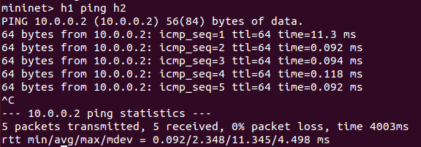
\includegraphics[width=1.00\textwidth]{./pictures/ping_test1_flood.png}
	\caption{Mininet Traffic ping from h1 to h2}
	\label{x}
	\end{center}
\end{figure} 

\subsubsection{Flow Table}
Wenn man die Flow Table anzeigen lässt sind jetzt mehrere Einträge vorhanden. Man erkennt daraus den Pfad mit Priorität 0: Controller, und den Pfad mit Priorität 1: Flood. Eine weitere wichtige Erkennung ist die Anzahl Pakete. Unter dem Eintrag mit Priorität 0 ist zu sehen das sich die Anzahl Pakete auf eines beschränkt, und der Pfad mit Priorität 1 die restlichen Pakete des flows enthält. 
\begin{figure} [H]
	\begin{center}
	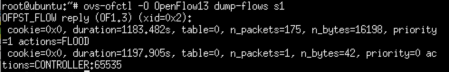
\includegraphics[width=1.00\textwidth]{./pictures/flow_table_flood.png}
	\caption{s1 flow table}
	\label{x}
	\end{center}
\end{figure} 
\newpage

\subsection{c0 flow}
Auf der Konsole des Controllers c0 ist ebenfalls ersichtlich das nur ein Paket zu ihm geschickt wird. 
\begin{figure} [H]
	\begin{center}
	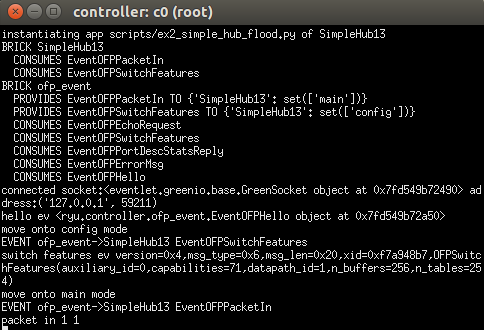
\includegraphics[width=0.60\textwidth]{./pictures/c0_ex2.png}
	\caption{c0 flow}
	\label{x}
	\end{center}
\end{figure} 

\subsubsection{Wireshark OpenFlow}
Im Wireshark ist ebenfalls ersichtlich, dass die Pakete auf allen Ports gefloodet werden. 
Nachdem das Erste Paket an den Controller gesendet wird, werden die restlichen auf allen Ports gefloodet. 
\begin{figure} [H]
	\begin{center}
	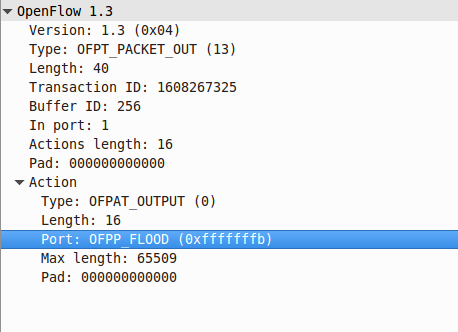
\includegraphics[width=0.60\textwidth]{./pictures/wireshark-flood.png}
	\caption{wireshark capture flooding}
	\label{x}
	\end{center}
\end{figure} 
\newpage

\section{Implementing a Switch}

\subsection{Aufgabe}
Wurde aus der Aufgabenstellung entnommen: \\
\\
Now you should be familiar with the functionality of the RYU SDN controller. In this exercise you will write a learning switch. This is more challenging than the hub implementation. The following steps should guide you:
\begin{itemize}
\item OpenFlow-Switch: Packet incoming\\
Existing flow?\\
No flow: send to controller
\item Learn source MAC address and incoming port
\item Write into table
\item  Destination MAC address already in table?\\
Yes, forward packet only to outgoing port: install flow on Switch\\
No, flood packet to all ports, except the incoming port
\item Existing flow
\item Forward as specified
\end{itemize}

\subsection{Ziel der Aufgabe}
In dieser Aufgabe soll jetzt ein Switch implementiert werden der die Pfade lernt. Falls der Switch noch keinen Flow für ein Paket hat, so soll er dieses zum Controller schicken. Der Switch soll sich neu die MAC-Adressen und den dazugehörigen Port merken. 

\subsection{Infrastruktur}
An der Infrastruktur ändert sich für diese Aufgabe nur das Script. Ansonsten dieselbe wie 1.1.3.
\newpage

\subsection{Script: Implementing a Switch}
\begin{lstlisting}
#!/usr/bin/env python
from ryu.base import app_manager
from ryu.controller import ofp_event
from ryu.controller.handler import CONFIG_DISPATCHER, MAIN_DISPATCHER
from ryu.controller.handler import set_ev_cls
from ryu.ofproto import ofproto_v1_3
from ryu.lib.packet import packet
from ryu.lib.packet import ethernet

class SimpleHub13(app_manager.RyuApp):
    OFP_VERSIONS = [ofproto_v1_3.OFP_VERSION]

    def __init__(self, *args, **kwargs):
        super(SimpleHub13, self).__init__(*args, **kwargs)

    @set_ev_cls(ofp_event.EventOFPSwitchFeatures, CONFIG_DISPATCHER)
    def switch_features_handler(self, ev):
        datapath = ev.msg.datapath
        ofproto = datapath.ofproto
        parser = datapath.ofproto_parser
        match = parser.OFPMatch()
        actions = [parser.OFPActionOutput(ofproto.OFPP_CONTROLLER, 
        		ofproto.OFPCML_NO_BUFFER)]
        self.add_flow(datapath, 0, match, actions)

    def add_flow(self, datapath, priority, match, actions):
        ofproto = datapath.ofproto
        parser = datapath.ofproto_parser
        inst = [parser.OFPInstructionActions(
        			ofproto.OFPIT_APPLY_ACTIONS, actions)]
        mod = parser.OFPFlowMod(datapath=datapath, priority=priority, 
        				match=match, instructions=inst)
        datapath.send_msg(mod)

    @set_ev_cls(ofp_event.EventOFPPacketIn, MAIN_DISPATCHER)
    def _packet_in_handler(self, ev):
        msg = ev.msg
        datapath = msg.datapath
        ofproto = datapath.ofproto
        parser = datapath.ofproto_parser
        in_port = msg.match['in_port']
        
                pkt = packet.Packet(msg.data)
        eth = pkt.get_protocols(ethernet.ethernet)[0]

        dst = eth.dst
        src = eth.src

        dpid = datapath.id
        self.mac_to_port.setdefault(dpid,{})

        self.logger.info("packet in %s %s %s %s", 
        		dpid, src, dst, in_port)

        self.mac_to_port[dpid][src] = in_port

        if dst in self.mac_to_port[dpid]:
            out_port = self.mac_to_port[dpid][dst]
        else:
            out_port = ofproto.OFPP_FLOOD

        actions = [parser.OFPActionOutput(out_port)]

        if out_port != ofproto.OFPP_FLOOD:
            match = parser.OFPMatch(in_port=in_port, eth_dst=dst)
            self.add_flow(datapath, 1, match, actions)
		
        data = None
        if msg.buffer_id == ofproto.OFP_NO_BUFFER:
            data = msg.data

        out = parser.OFPPacketOut(datapath=datapath, 
        	buffer_id=msg.buffer_id, in_port=in_port, 
        		actions=actions, data=data)
        datapath.send_msg(out)
        dpid = datapath.id
\end{lstlisting}
\newpage

\subsection{Traffic}
Mittels Wireshark sollte jetzt das Resultat nachvollziehbar sein. Wir haben einen Test durchgeführt mittels einem Ping von h1 zu h2. 

\subsubsection{Wireshark: first packet in}
Das Erste Paket wird an den Controller gesendet, da der flow nicht bekannt ist. 
\begin{figure} [H]
	\begin{center}
	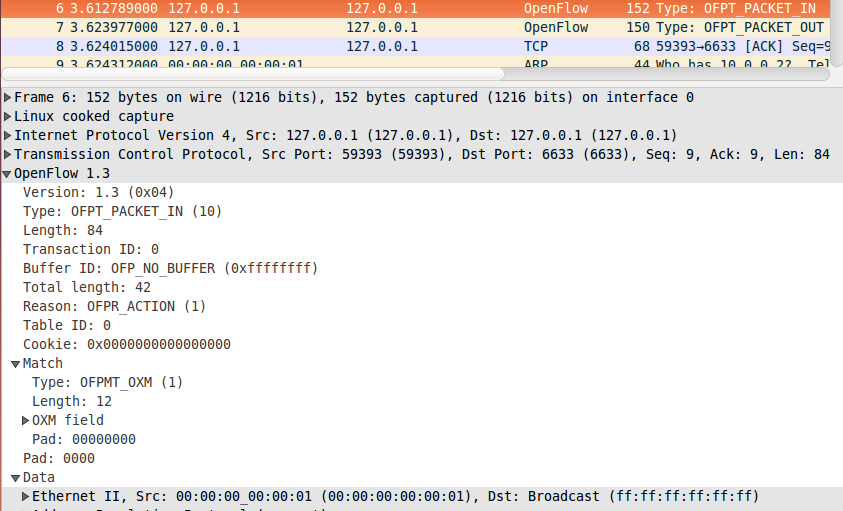
\includegraphics[width=0.80\textwidth]{./pictures/ex3_paket_in.png}
	\caption{wireshark capture first packet in}
	\label{x}
	\end{center}
\end{figure} 

\subsubsection{Wireshark: first packet in - packet out flood}
Da der flow nicht bekannt ist, wird als packet out einen flood durchgeführt 
\begin{figure} [H]
	\begin{center}
	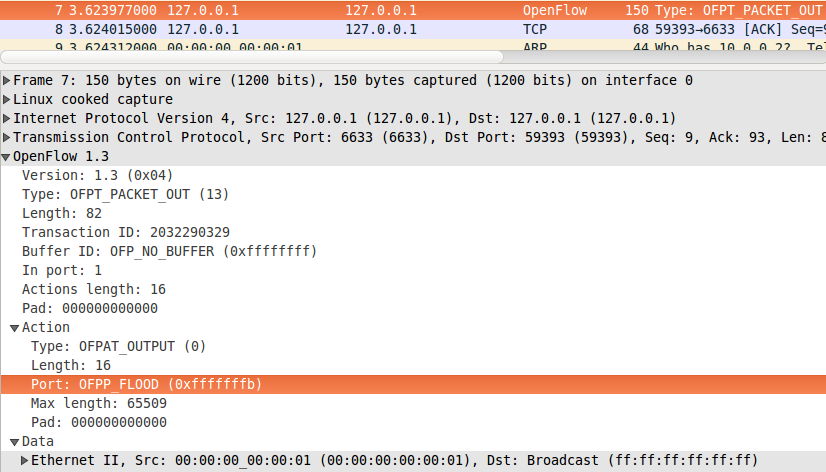
\includegraphics[width=0.70\textwidth]{./pictures/ex3_paket_out.png}
	\caption{wireshark capture packet out flood}
	\label{x}
	\end{center}
\end{figure} 

\subsubsection{Wireshark: packet out learning port}
Jetzt learnt der Switch den flow und merkt sich die MAC-Adresse und den dazugehörigen Port. 
\begin{figure} [H]
	\begin{center}
	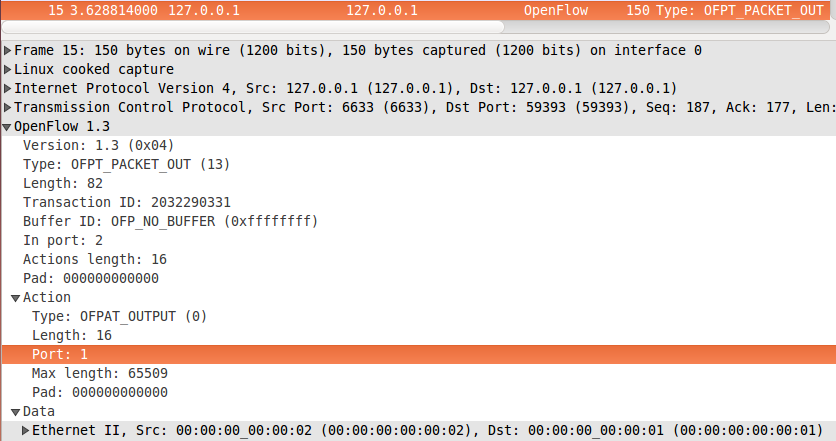
\includegraphics[width=0.80\textwidth]{./pictures/ex3_paket_out_port.png}
	\caption{wireshark capture learning port}
	\label{x}
	\end{center}
\end{figure} 

\subsubsection{Wireshark: traffic direct after learning}
Nachdem die MAC-Adresse und den dazugehörgen Port bekannt ist, verläuft der traffic direkt. 
\begin{figure} [H]
	\begin{center}
	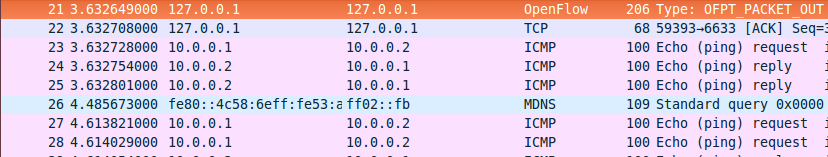
\includegraphics[width=0.80\textwidth]{./pictures/ex3_paket_direct.png}
	\caption{wireshark capture direct traffic}
	\label{x}
	\end{center}
\end{figure} 
\newpage

\section{Implementing a policy-based controller}

\subsection{Aufgabenstellung}
Wurde aus der Aufgabenstellung entnommen: \\
\\
In this exercise you will implement a controller which allows or denies traffic based on a specified policy.
\begin{figure} [H]
	\begin{center}
	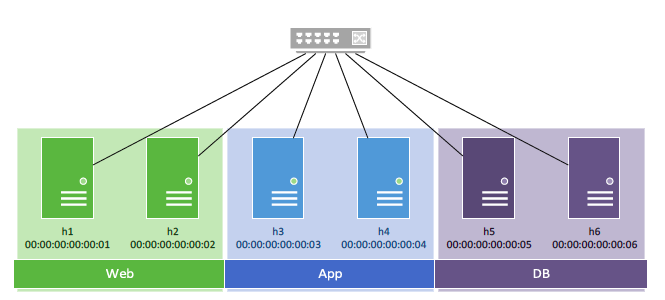
\includegraphics[width=0.80\textwidth]{./pictures/ex4_aufgabenstellung.png}
	\caption{ex4 Aufgabenstellung}
	\label{x}
	\end{center}
\end{figure} 
\noindent Each Server tenant can reach only the allowed tenants. (Web <> App, App <> DB)
Start Mininet: 
\begin{lstlisting}
sudo mn --topo single, 6 --mac --controller remote, ip=127.0.0.1
\end{lstlisting}
You can test your script with h1 ping h2 or pingall in the mininet CLI. h1 xterm opens a new
terminal for host h1. Now you can use for example tcpdump.
The second pingall output should looks like this:
\begin{figure} [H]
	\begin{center}
	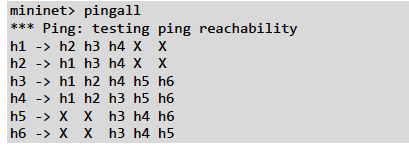
\includegraphics[width=0.80\textwidth]{./pictures/ex4_aufgabenstellung2.png}
	\caption{ex4 Aufgabenstellung}
	\label{x}
	\end{center}
\end{figure} 
\newpage
\noindent The minimal script must work with this fixed Topology. We will test your script with our Docker
container and 
\begin{lstlisting}
sudo mn --topo single,6 --mac --controller remote, ip=127.0.0.1
\end{lstlisting}
Optional you can add more flexibility with csv files or a db.

\subsubsection{Appendix: Quickstart}
\begin{itemize}
\item To get started, start your VM or private Linux. You can install Ryu or use our Docker container.
\item Run Mininet on a terminal window using the following command. This starts a network emulation environment to emulate 1 switch with 3 hosts.
\end{itemize} 
\begin{lstlisting}
sudo mn --topo single,3 --mac --controller remote
\end{lstlisting}
\begin{itemize}
\item The above command will spawn 1 switch that has support for both OpenFlow ver 1.0 and 1.3. Based on your needs, however, you can force a switch to support OpenFlow 1.3 by executing this command:
\end{itemize}
\begin{lstlisting}
sudo ovs-vsctl set Bridge s1 protocols=OpenFlow13
\end{lstlisting}
\begin{itemize}
\item Next, start the RYU Controller.
\end{itemize}
\begin{figure} [H]
	\begin{center}
	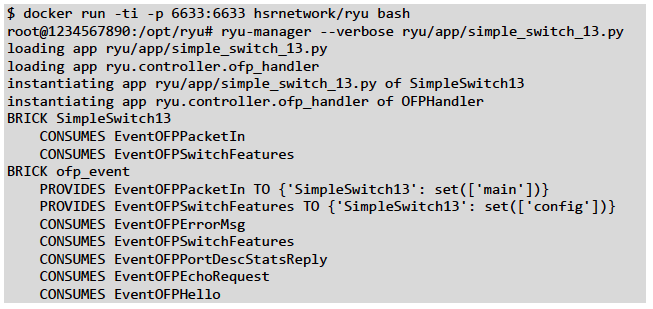
\includegraphics[width=1.00\textwidth]{./pictures/ex4_aufgabenstellung3.png}
	\caption{ex4 Aufgabenstellung}
	\label{x}
	\end{center}
\end{figure} 
\newpage
\begin{itemize}
\item Ensure that we start the correct ryu-manager if multiple versions of the controller is installed in the same system.
\item Have you changed the OpenFlow version on bridge s1?
\item Next, check if the hosts in the mininet topology can reach each other
\end{itemize}
\begin{figure} [H]
	\begin{center}
	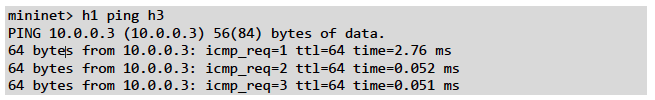
\includegraphics[width=1.00\textwidth]{./pictures/ex4_aufgabenstellung4.png}
	\caption{ex4 Aufgabenstellung}
	\label{x}
	\end{center}
\end{figure} 

\subsubsection{ryu code structure}
The main controller code is organized under the /ryu/ folder (In our Docker – /opt/ryu/ryu/). Here we discuss the functionalities of the key components. It is important to become familiar with them.
\begin{itemize}
\item app/ – Contains set of applications that run on-top of the controller.
\item base/ – Contains the base class for RYU applications. The RyuApp class in the appmanager.py file is inherited when creating a new application.
\item controller/ – Contains the required set of files to handle OpenFlow functions (e.g., packets from switches, generating flows, handling network events, gathering statistics etc).
\item lib/ – Contains set of packet libraries to parse different protocol headers and a library for OFConfig. In addition, it includes parsers for Netflow and sFlow too.
\item ofproto/ – Contains the OpenFlow protocol specific information and related parsers to support different versions of OF protocol (1.0, 1.2, 1.3, 1.4)
\item topology/: Contains code that performs topology discovery related to OpenFlow switches and handles associated information (e.g., ports, links etc). Internally uses LLDP protocol.
\end{itemize}

\subsubsection{ryu	controller code essentials}
Most controller platforms expose some native features to allow these key features:
\begin{itemize}
\item Ability to listen to asynchronous events (e.g., PACKET\_IN, FLOW\_REMOVED) and to observe events using ryu.controller.handler.set\_ev\_cls decorator.
\item Ability to parse incoming packets (e.g., ARP, ICMP, TCP) and fabricate packets to send out into the network
\item Ability to create and send an OpenFlow SDN message (e.g., PACKET\_OUT, FLOW\_MOD, STATS\_REQUEST) to the programmable dataplane.
\end{itemize}
With RYU you can achieve all of those by invoking set of applications to handle network events, parse any switch request and react to network changes by installing new flows, if required. For instance, creating a new application involves creating a subclass of RyuApp and building the required logic to listen for network events.\\
https://github.com/osrg/ryu/blob/master/ryu/ofproto/ofproto\_v1\_3.py\\
Line 234: enum ofp\_action\_type Line 1138: Match Fields \\
https://github.com/osrg/ryu/blob/master/ryu/ofproto/ofproto\_v1\_3\_parser.py\\
Events: EventOFPErrorMsg, EventOFPEchoRequest, EventOFPEchoReply, EventOFPSwitchFeatures, EventOFPGetConfigReply, EventOFPPacketIn, EventOFPFlowRemoved, EventOFPPortStatus, EventOFPDescStatsReply, EventOFPFlowStatsReply, EventOFPAggregateStatsReply, EventOFPTableStatsReply, EventOFPPortStatsReply, EventOFPQueueStatsReply, EventOFPGroupStatsReply, EventOFPGroupDescStatsReply, EventOFPGroupFeaturesStatsReply, EventOFPMeterStatsReply, EventOFPMeterConfigStatsReply, EventOFPMeterFeaturesStatsReply, EventOFPPortDescStatsReply, EventOFPBarrierReply, EventOFPQueueGetConfigReply, EventOFPRoleRepl, EventOFPGetAsyncReply

\subsection{Ziel der Aufgabe}
Auf dem Controllen sollen Policys erstellt werden, welche bestimmen, welcher Host mit welchem kommunizieren darf. 

\subsection{Infrastruktur}
An der Infrastruktur ändert sich für diese Aufgabe nur das Script. Ansonsten dieselbe wie 1.1.3.

\subsection{Start Mininet und Vorbereitung}
Für diese Aufgabe werden 6 Hosts benötigt. Mininet muss mit folgendem Befehl gestartet werden.
\begin{lstlisting}
sudo mn --topo single,6 --mac --controller remote,ip=127.0.0.1 
\end{lstlisting}
Ebenfalls muss OpenFlow13 auf dem s1 aktiviert sein: 
\begin{lstlisting}
s1: ovs-vsctl set bridge s1 protocols=OpenFlow13
\end{lstlisting}
Der ryu-manager kann wie bisher gestartet werden mit dem neuem Script: 
\begin{lstlisting}
c0: ryu-manager --verbose scripts/ex4_controller_policy.py
\end{lstlisting}

\subsubsection{ACL}
Gemäss Aufgabe dürfen nicht alle Hosts miteinander kommunizieren. 
\begin{itemize}
\item h1 --> h2,h3,h4 (group1)
\item h2 --> h1,h3,h4 (group2)
\item h3 --> h1,h2,h4,h5,h6 (group3)
\item h4 --> h1,h2,h3,h5,h6 (group4)
\item h5 --> h3,h4,h6 (group5)
\item h6 --> h3,h4,h5 (group6)
\end{itemize}

\subsection{Script: Policy-based controller}
\begin{lstlisting}
#!/usr/bin/env python
from ryu.base import app_manager
from ryu.controller import ofp_event
from ryu.controller.handler import CONFIG_DISPATCHER, MAIN_DISPATCHER
from ryu.controller.handler import set_ev_cls
from ryu.ofproto import ofproto_v1_3
from ryu.lib.packet import packet
from ryu.lib.packet import ethernet
         
class PolicyController(app_manager.RyuApp):
    OFP_VERSIONS = [ofproto_v1_3.OFP_VERSION]
    
    #Definition Host MAC-Adressen inkl. Broadcast
    h1 = '00:00:00:00:00:01'
    h2 = '00:00:00:00:00:02'
    h3 = '00:00:00:00:00:03'
    h4 = '00:00:00:00:00:04'
    h5 = '00:00:00:00:00:05'
    h6 = '00:00:00:00:00:06'
    broadcast = 'ff:ff:ff:ff:ff:ff'
    
    #Definition Access Gruppen - Bsp.: h1 kann mit group1 kommunizieren
    group1 = ["00:00:00:00:00:02","00:00:00:00:00:03",
    	"00:00:00:00:00:04"]
    group2 = ["00:00:00:00:00:01","00:00:00:00:00:03",
    	"00:00:00:00:00:04"]
    group3 = ["00:00:00:00:00:01","00:00:00:00:00:02",
    	"00:00:00:00:00:04","00:00:00:00:00:05","00:00:00:00:00:06"]
    group4 = ["00:00:00:00:00:01","00:00:00:00:00:02",
    	"00:00:00:00:00:03","00:00:00:00:00:05","00:00:00:00:00:06"]
    group5 = ["00:00:00:00:00:03","00:00:00:00:00:04",
    	"00:00:00:00:00:06"]
    group6 = ["00:00:00:00:00:03","00:00:00:00:00:04",
    	"00:00:00:00:00:05"]

    print "----------------"

    print "Host 1", h1
    print "Host 2", h2
    print "Host 3", h3
    print "Host 4", h4
    print "Host 5", h5
    print "Host 6", h6

    print "Access Group Host1", group1
    print "Access Group Host2", group2
    print "Access Group Host3", group3
    print "Access Group Host4", group4
    print "Access Group Host5", group5
    print "Access Group Host6", group6    
    
    print "----------------"

    def __init__(self, *args, **kwargs):
        super(PolicyController, self).__init__(*args, **kwargs)
        self.mac_to_port = {}

    @set_ev_cls(ofp_event.EventOFPSwitchFeatures, CONFIG_DISPATCHER)
    def switch_features_handler(self, ev):
        datapath = ev.msg.datapath
        ofproto = datapath.ofproto
        parser = datapath.ofproto_parser
        match = parser.OFPMatch()
        actions = [parser.OFPActionOutput(ofproto.OFPP_CONTROLLER, 
        	ofproto.OFPCML_NO_BUFFER)]
        self.add_flow(datapath, 0, match, actions)

    def add_flow(self, datapath, priority, match, actions):
        ofproto = datapath.ofproto
        parser = datapath.ofproto_parser
        inst = [parser.OFPInstructionActions(
        	ofproto.OFPIT_APPLY_ACTIONS, actions)]
        mod = parser.OFPFlowMod(datapath=datapath, priority=priority, 
        	match=match, instructions=inst)
        datapath.send_msg(mod)

    @set_ev_cls(ofp_event.EventOFPPacketIn, MAIN_DISPATCHER)
    def _packet_in_handler(self, ev):
        msg = ev.msg
        datapath = msg.datapath
        ofproto = datapath.ofproto
        parser = datapath.ofproto_parser
        in_port = msg.match['in_port']

        pkt = packet.Packet(msg.data)
        eth = pkt.get_protocols(ethernet.ethernet)[0]

        dst = eth.dst
        src = eth.src

        dpid = datapath.id
        self.mac_to_port.setdefault(dpid,{})

        self.logger.info("packet in %s %s %s %s", 
        	dpid, src, dst, in_port)

        self.mac_to_port[dpid][src] = in_port

	print "-------------------"

	print "source address:", src
	print "destination address:", dst

	print "-------------------"

	actions = []
	out_port = ""

        if src == self.h1 and dst in self.group1[0:]:   
	    print "Fall 1: h1 ping to group1"
	    out_port = self.mac_to_port[dpid][dst]
            actions = [parser.OFPActionOutput(out_port)]
            match = parser.OFPMatch(in_port=in_port,eth_dst=dst)
            self.add_flow(datapath, 1, match, actions)
            self.logger.info("access allowed %s %s", src, dst)
        elif src == self.h2 and dst in self.group2[0:]:
            print "Fall 2: h2 ping to group2"
            out_port = self.mac_to_port[dpid][dst]
            actions = [parser.OFPActionOutput(out_port)]
            match = parser.OFPMatch(in_port=in_port,eth_dst=dst)
            self.add_flow(datapath, 1, match, actions)
            self.logger.info("access allowed %s %s", src, dst)
        elif src == self.h3 and dst in self.group3[0:]:
            print "Fall 3: h3 ping to group3"
            out_port = self.mac_to_port[dpid][dst]
            actions = [parser.OFPActionOutput(out_port)]
            match = parser.OFPMatch(in_port=in_port,eth_dst=dst)
            self.add_flow(datapath, 1, match, actions)
            self.logger.info("access allowed %s %s", src, dst)
        elif src == self.h4 and dst in self.group4[0:]:
            print "Fall 4: h4 ping to group4"
            out_port = self.mac_to_port[dpid][dst]
            actions = [parser.OFPActionOutput(out_port)]
            match = parser.OFPMatch(in_port=in_port,eth_dst=dst)
            self.add_flow(datapath, 1, match, actions)
            self.logger.info("access allowed %s %s", src, dst)
        elif src == self.h5 and dst in self.group5[0:]:
            print "Fall 5: h5 ping to group5"
            out_port = self.mac_to_port[dpid][dst]
            actions = [parser.OFPActionOutput(out_port)]
            match = parser.OFPMatch(in_port=in_port,eth_dst=dst)
            self.add_flow(datapath, 1, match, actions)
            self.logger.info("access allowed %s %s", src, dst)
        elif src == self.h6 and dst in self.group6[0:]:
            print "Fall 6: h6 ping to group6"
            out_port = self.mac_to_port[dpid][dst]
            actions = [parser.OFPActionOutput(out_port)]
            match = parser.OFPMatch(in_port=in_port,eth_dst=dst)
            self.add_flow(datapath, 1, match, actions)
            self.logger.info("access allowed %s %s", src, dst)        
	elif dst == self.broadcast:
	    print "Fall 7: destination is broadcast " 
            out_port = ofproto.OFPP_FLOOD
	    match = [parser.OFPMatch(in_port=in_port, eth_dst=dst)]
	    actions = [parser.OFPActionOutput(out_port)]
            self.logger.info("broadcast detect %s %s", src, dst)
        else:
	    print "Fall 8: no match" 
            self.logger.info("access denied %s %s", src, dst)

        data = None
        if msg.buffer_id == ofproto.OFP_NO_BUFFER:
            data = msg.data

        out = parser.OFPPacketOut(datapath=datapath, buffer_id=
        	msg.buffer_id, in_port=in_port, actions=actions, 
        		data=data)
        datapath.send_msg(out)
        dpid = datapath.id

\end{lstlisting}

\subsection{Beschreibung zu Script}
Unser Script arbeitet mit keinem Import einer Liste, sondern mit Variablen und Arrays. Die Host MAC-Adressen werden als Variablen definiert und die jeweiligen ACLs der Hosts, sind Arrays mit den jeweiligen Client MAC-Adressen als Inhalt. Beispiel: h1 kann mit allen MAC-Adressen die in group1 eingetragen sind kommunizieren. Diese Abfrage passiert in den untenstehenden IF-Abfragen. Es gibt insgesamt 8 Fälle: 1-6 sind Fälle von erlaubten Zugriffen (h1-h6 auf group1-group6), ein Fall betrifft der Broadcast und der letzte Fall betrifft keinen match (Zugriff verweigert). Eine Erweiterungsmöglichkeit wäre es das Gesamte skalierbar zu implementieren, mit Hilfe einer externen Liste. 

\subsection{Traffic}
In diesem Kapitel zeigen wir diverse Traffic Verhalten von unserer Infrastruktur. 

\subsubsection{Pingall}
Mit pingall kann auf Mininet die gesamte Implementation getestet werden. Die Hosts müssten gemäss Kapitel ACL miteinander kommunizieren können, oder auch nicht. 
\begin{figure} [H]
	\begin{center}
	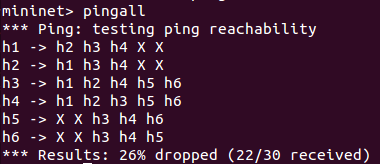
\includegraphics[width=0.60\textwidth]{./pictures/pingall.png}
	\caption{pingall mininet}
	\label{x}
	\end{center}
\end{figure} 
Gemäss Aussage von dieser Abbildung funktioniert der Aufbau wie gefodert. 

\subsubsection{c0 flow}
Was zeigt der Controller auf der Konsole während dem traffic fliesst? Hier einen Auszug von unserem c0 Controller. Wir zeigen nicht den gesamten Konsolenauszug, da dieser enorm lang ist. Wir haben die wichtigsten Positionen im Script mit Ausgaben geschmückt, damit man das Verhalten besser nachvollziehen kann. Wir zeigen einmal ein erfolgreicher Ping von h1 zu h2, und ein nicht erlaubter Ping von h1 zu h6. 
\begin{itemize}
\item mininet: h1 ping h2 (allowed)
\begin{figure} [H]
	\begin{center}
	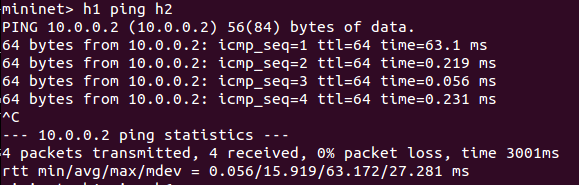
\includegraphics[width=0.70\textwidth]{./pictures/h1_ping_h2_ok.png}
	\caption{erfolgreicher ping von h1 zu h2}
	\label{x}
	\end{center}
\end{figure} 
\begin{figure} [H]
	\begin{center}
	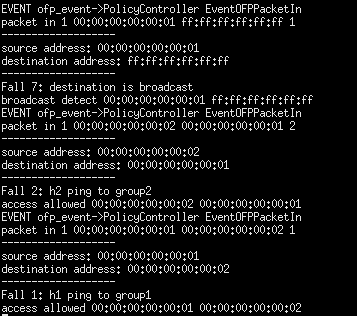
\includegraphics[width=0.80\textwidth]{./pictures/h1_ping_h2.png}
	\caption{c0 flow bei allowed access}
	\label{x}
	\end{center}
\end{figure} 
\item mininet: h1 ping h6 (not allowed)
\begin{figure} [H]
	\begin{center}
	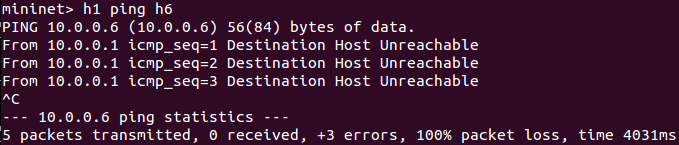
\includegraphics[width=0.70\textwidth]{./pictures/h1_ping_h6_nok.png}
	\caption{kein erfolgreicher ping von h1 zu h6}
	\label{x}
	\end{center}
\end{figure} 
\begin{figure} [H]
	\begin{center}
	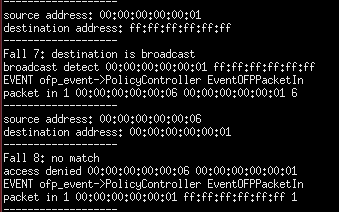
\includegraphics[width=0.70\textwidth]{./pictures/h1_ping_h6.png}
	\caption{c0 flow bei access denied}
	\label{x}
	\end{center}
\end{figure} 
\end{itemize}

\subsubsection{s1 flow table}
In der flow table kann man die jeweiligen bereits bekannten Pfade anzeigen lassen. Gemäss diesem Bild ist der Pfad zu h1,h2 und h3 bereits bekannt. Jeder neue traffic der an diese drei Hosts adressiert ist, wird nicht mehr zum Controller c0 geschickt. 
\begin{figure} [H]
	\begin{center}
	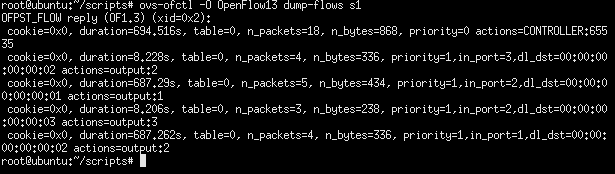
\includegraphics[width=0.80\textwidth]{./pictures/ex4_flow_table.png}
	\caption{s1 flow table}
	\label{x}
	\end{center}
\end{figure} 

\subsubsection{Wireshark: first traffic - flood}
Bei einem unbekannten flow (immer bei der Ersten Kontaktaufnahme) wird gefloodet. Das ist der Fall 7 in im Python Script. 
\begin{figure} [H]
	\begin{center}
	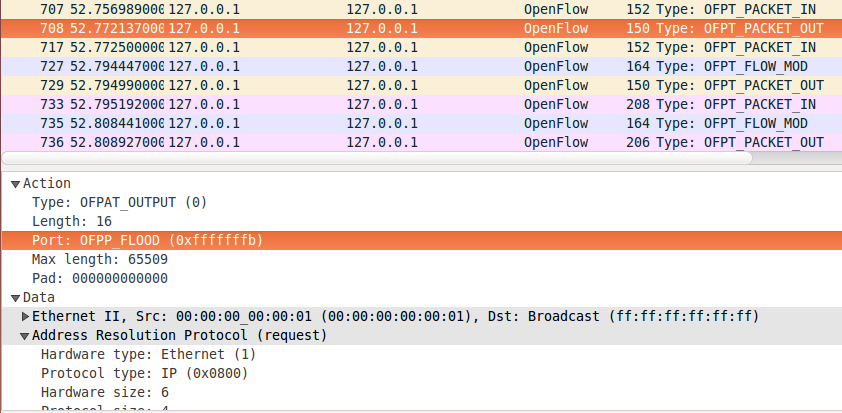
\includegraphics[width=0.80\textwidth]{./pictures/ex4_packet_flood.png}
	\caption{first traffic - flood}
	\label{x}
	\end{center}
\end{figure} 

\subsubsection{Wireshark: allowed flow}
Kontaktiert h1 einen erlaubten Host so werden folgende Einträge angezeigt. Das Feld Actions enthält die zu durchführende Aktion. 
\begin{figure} [H]
	\begin{center}
	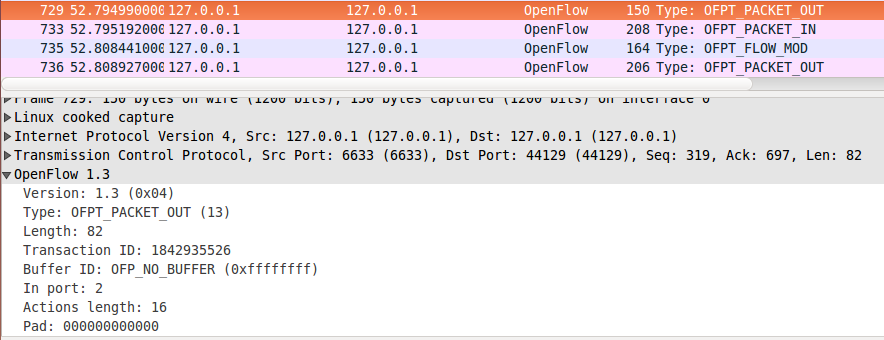
\includegraphics[width=0.80\textwidth]{./pictures/ex4_packet_action.png}
	\caption{allowed flow}
	\label{x}
	\end{center}
\end{figure} 
\begin{figure} [H]
	\begin{center}
	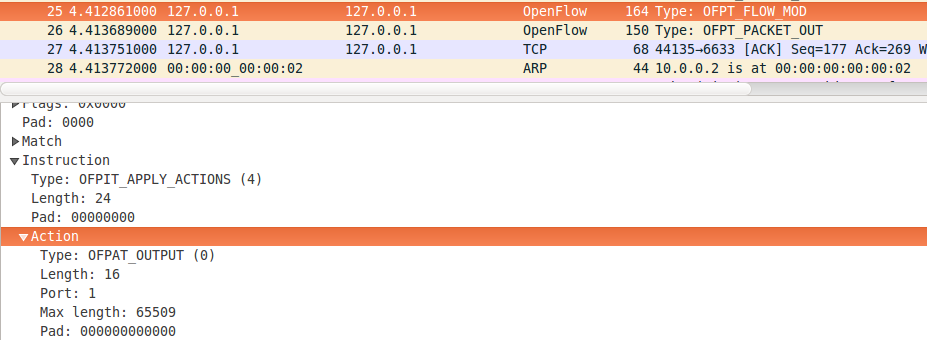
\includegraphics[width=0.80\textwidth]{./pictures/ex4_packet_action2.png}
	\caption{allowed flow}
	\label{x}
	\end{center}
\end{figure} 

\subsubsection{Wireshark: denied flow}
Wird einen nicht erlaubten flow aufgebaut, so bleibt das Feld Actions leer. Die Pakete werden verworfen. 
\begin{figure} [H]
	\begin{center}
	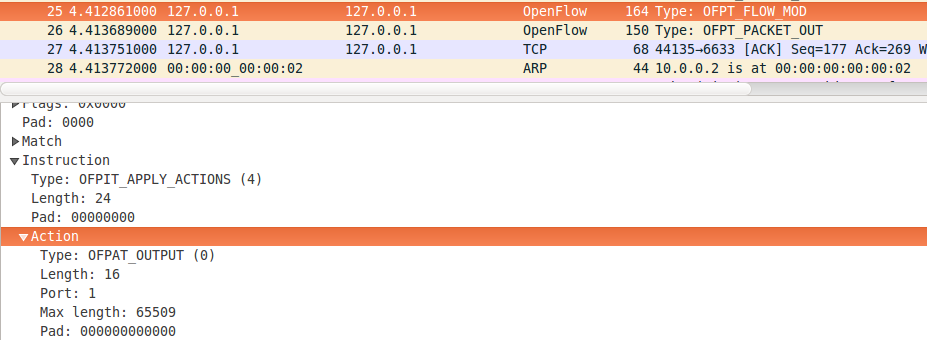
\includegraphics[width=0.80\textwidth]{./pictures/ex4_packet_action2.png}
	\caption{access denied, drop packet}
	\label{x}
	\end{center}
\end{figure} 

\section{Referenzen}
Als Referenz für diese Arbeit wurde das ryubook.pdf verwendet. 
\end{document}